\section{簡介}
  前一章介紹的支撐向量機至今已經是一個被廣泛使用的機器學習模型,
  它在二元分類問題上的表現往往十分突出,
  甚至有不少人因此視它為最好的學習模型。
  正由於支撐向量機在二元分類上的表現突出,
  所以支撐向量機在多元分類(Multiclass Classification)問題上也是用二元分類來擴充的。
  支撐向量機的多元分類有兩種作法:
  假設我們有$n$個類別,
  一種作法是訓練區別兩兩不同類別的支撐向量機(共$\binom{n}{2}$),
  當一個新的樣本點進來我們就用這$\binom{n}{2}$個支撐向量機表決。
  (我們稱這種叫一對一(One Versus One))
  另一種作法則是訓練區分第$k$個類別跟其他類別的支撐向量機(共$n$個),
  當新的樣本點進來,
  我們就用這$n$個支撐向量機都跑一次然後選分數最大的那個類別。
  (這種叫做一對多(One Versus All))。

  儘管在支撐向量機在多元分類問題上已經有擴充,
  但像支撐向量機這樣屬於統計學派(Statistical School)的模型,
  在碰到像語音辨識或是語句解析(Parsing)這種輸出具有結構性的問題,
  (語音辨識的輸出是一長串符號、語句解析的輸出是一棵解析樹(Parse Tree))
  往往就只能舉手投降,
  將問題讓給貝氏學派(Bayesian School)的模型。
  
  不過,
  近年來對於結構性輸出的問題,
  統計學派的模型似乎露出一線曙光。
  結構化支撐向量機(Structural Support Vector Machine; SVM-struct)\cite{SVMstruct}就是一個例子。
  為了說明結構化支撐向量機,
  我們先來定義一些符號。
  
  假設我們希望學習的是一個函數$f$將特徵向量$x \in \mathcal{X}$映到$y \in \mathcal{Y}$。
  跟傳統的支撐向量機不同的是,
  $y$不是$\lbrace -1, 1 \rbrace$這樣的二元標籤,
  也不是$\lbrace 1, 2, \ldots k \rbrace$這樣的$k$元標籤。
  而是有結構性的元素,
  像是一個序列(Sequence)、字串(String)、樹(Tree)、甚至是一般圖(Graph)(但必須是離散的空間)。
  舉例來說,
  考慮自然語言處理中的語句分析,
  我們要學的$f$就是將一個句子$x$從語句空間(所有可能的語句所組成),
  映到一棵解析樹$y$(Parse Tree)。
  因此,
  假設我們有的訓練集是
  \begin{equation}
    Z = (x_i, y_i)_{i=1}^n 
  \end{equation}
  在這個例子$x_i$就是每個樣本語句,
  以及它對應我們認為正確的解析樹$y_i$。

\section{原始形式(Primal Form)及對偶形式(Dual Form)}
  要將支撐向量機直接按照多元分類問題的方式擴充到結構性輸出的問題上是不可能的,
  因為如果把每一個不同結構性輸出都當作一種分類的話,
  這樣組合起來的數量就有指數級別。
  我們必須想辦法繞過這個困境。

  我們嘗試從多元分類中得到一些靈感。
  先不要管指數級別的問題,
  假設我們用一對多的多元分類方式來做我們的結構性輸出預測。
  也就是說每一個類別都有自己訓練的一組$w$。
  當我們做分類的時候,
  就是將輸入$x$對每一組$w$都做一次內積,
  然後按照分數從高到低排序。
  (如圖\ref{fig:multiple_svm_rank},
  從$w_1$到$w_9$代表不同的9個類別的$w$,位置越高表示算出來的分數越高。
  由於圖中$w_4$分數最高,
  所以最後輸出的預測是第四個類別)
  \begin{figure}
    \begin{center}
      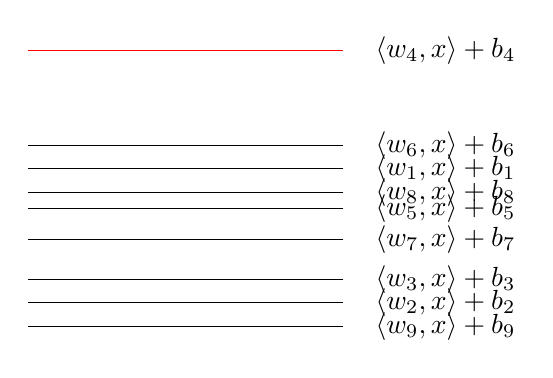
\begin{tikzpicture}[scale=1]
	\draw (0.5,0.5) -- (4.5,0.5);
	\draw (0.5,0.8) -- (4.5,0.8);
	\draw (0.5,1.1) -- (4.5,1.1);
	\draw (0.5,1.6) -- (4.5,1.6);
	\draw (0.5,2) -- (4.5,2);
	\draw (0.5,2.2) -- (4.5,2.2);
	\draw (0.5,2.5) -- (4.5,2.5);
	\draw (0.5,2.8) -- (4.5,2.8);
	\draw[red] (0.5,4) -- (4.5,4);
	\draw (5.8, 0.5) node {$\langle w_9, x \rangle + b_9$}; 
	\draw (5.8, 0.8) node {$\langle w_2, x \rangle + b_2$};
	\draw (5.8, 1.1) node {$\langle w_3, x \rangle + b_3$};
	\draw (5.8, 1.6) node {$\langle w_7, x \rangle + b_7$};
	\draw (5.8, 2) node {$\langle w_5, x \rangle + b_5$};
	\draw (5.8, 2.2) node {$\langle w_8, x \rangle + b_8$}; 
	\draw (5.8, 2.5) node {$\langle w_1, x \rangle + b_1$}; 
	\draw (5.8, 2.8) node {$\langle w_6, x \rangle + b_6$}; 
	\draw (5.8, 4) node {$\langle w_4, x \rangle + b_4$}; 
      \end{tikzpicture}
      \caption{一對多多元分類}
      \label{fig:multiple_svm_rank}
    \end{center}
  \end{figure}
  然後挑分數最高的那個分類作為我們的預測。

  我們可以這樣詮釋我們的分類方式。
  當我們考慮一個輸入$x \in \mathcal{X}$時,
  其實我們對所有結構性的$y \in \mathcal{Y}$作為$x$的答案是擁有某種偏好的($y$看作是某一個分類)。
  只是,
  我們在多元分類問題中表達偏好的方式是對每一個$y$都有一組不同的$w$來幫助我們決定偏好$\langle w, x \rangle + b$,
  這樣參數的量會隨著$y$呈指數成長。
  為了控制參數成長,
  我們引進特徵函數$\Psi(x, y)$,
  (等價於條件隨機域(Conditional Random Fields; CRF)中的特徵函數(Feature Function),
  用來表達$x$和$y$之間的某種關係。
  而$\Psi$的實際定義要看我們要應付的問題是什麼),
  將我們的偏好定義為$\langle w, \Psi(x, y) \rangle$。
  因此,
  $w$就是對應於某個特徵的權重,
  而$w$的維度就等於我們定義的特徵函數輸出的維度,
  也就是說參數量是固定的。

  說了這麼多,
  其實我們只是要定義一個參數量固定的鑑別函數(Discriminant Function)$F: \mathcal{X} \times \mathcal{Y} \longrightarrow \mathcal{R}$
  好表達我們對於$x$配上不同結構性輸出$y$有不同的偏好。
  這個鑑別函數可以看作是一個衡量$x$跟$y$匹配性的函數。
  當一組$(x, y)$透過$F$映到較大的實數時,
  表示他們是比較相配的,
  也就是我們偏好$y$作為$x$的答案。

  我們為什麼要一個參數化、衡量我們偏好的鑑別函數呢?
  如圖\ref{fig:fit_before_svm_struct}跟圖\ref{fig:fit_svm_struct}
  (圖中每一欄代表$F(x, y; w)$中固定一個$x$,
  而一欄中每一條線代表不同的$y$跟$x$的契合度。
  位置越高就代表$x$跟$y$間越契合。
  而紅色的線所對應的$y$就是我們訓練集中所給作是$x$答案的$y$,
  我們希望調整參數$w$,
  讓每一欄中的排序,
  紅色的線都排在第一名,
  且遠遠超過第二名,
  就像圖\ref{fig:fit_before_svm_struct}變成圖\ref{fig:fit_svm_struct}一樣)。
  \begin{figure}
    \begin{center}
      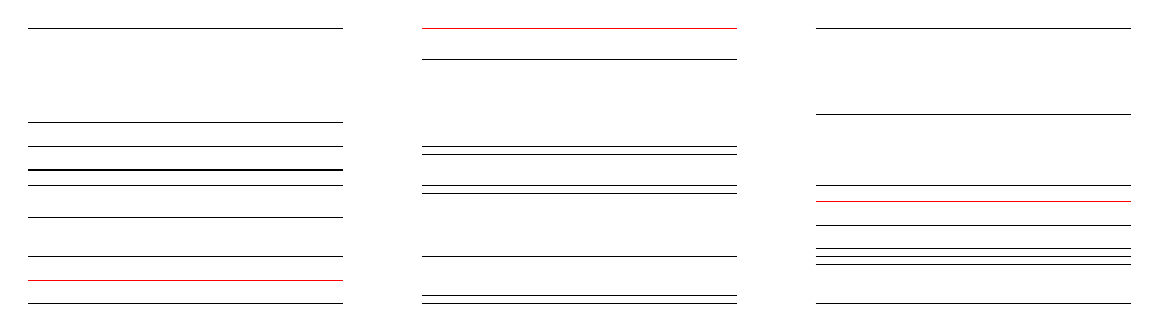
\begin{tikzpicture}[scale=1]
	\draw (0.5,0.5) -- (4.5,0.5);
	\draw[red] (0.5,0.8) -- (4.5,0.8);
	\draw (0.5,1.1) -- (4.5,1.1);
	\draw (0.5,1.6) -- (4.5,1.6);
	\draw (0.5,2) -- (4.5,2);
	\draw (0.5,2.2) -- (4.5,2.2);
	\draw (0.5,2.5) -- (4.5,2.5);
	\draw (0.5,2.8) -- (4.5,2.8);
	\draw (0.5,4) -- (4.5,4);
	
	\draw (5.5,0.5) -- (9.5,0.5);
	\draw (5.5,0.6) -- (9.5,0.6);
	\draw (5.5,1.1) -- (9.5,1.1);
	\draw (5.5,1.9) -- (9.5,1.9);
	\draw (5.5,2) -- (9.5,2);
	\draw (5.5,2.4) -- (9.5,2.4);
	\draw (5.5,2.5) -- (9.5,2.5);
	\draw (5.5,3.6) -- (9.5,3.6);
	\draw[red] (5.5,4) -- (9.5,4);
	
	\draw (10.5,0.5) -- (14.5,0.5);
	\draw (10.5,1) -- (14.5,1);
	\draw (10.5,1.1) -- (14.5,1.1);
	\draw (10.5,1.2) -- (14.5,1.2);
	\draw (10.5,1.5) -- (14.5,1.5);
	\draw[red] (10.5,1.8) -- (14.5,1.8);
	\draw (10.5,2) -- (14.5,2);
	\draw (10.5,2.9) -- (14.5,2.9);
	\draw (10.5,4) -- (14.5,4);
      \end{tikzpicture}
      \caption{調整$w$前所決定的鑑別函數}
      \label{fig:fit_before_svm_struct}
    \end{center}
  \end{figure}
  
  \begin{figure}
    \begin{center}
      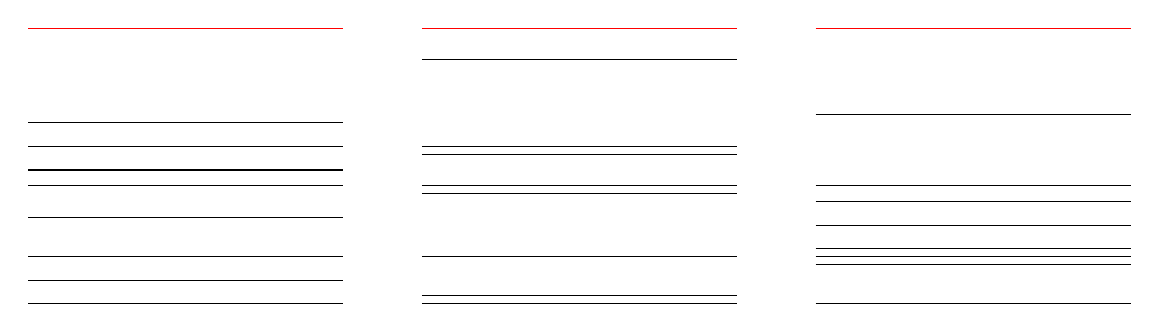
\begin{tikzpicture}[scale=1]
	\draw (0.5,0.5) -- (4.5,0.5);
	\draw (0.5,0.8) -- (4.5,0.8);
	\draw (0.5,1.1) -- (4.5,1.1);
	\draw (0.5,1.6) -- (4.5,1.6);
	\draw (0.5,2) -- (4.5,2);
	\draw (0.5,2.2) -- (4.5,2.2);
	\draw (0.5,2.5) -- (4.5,2.5);
	\draw (0.5,2.8) -- (4.5,2.8);
	\draw[red] (0.5,4) -- (4.5,4);
	
	\draw (5.5,0.5) -- (9.5,0.5);
	\draw (5.5,0.6) -- (9.5,0.6);
	\draw (5.5,1.1) -- (9.5,1.1);
	\draw (5.5,1.9) -- (9.5,1.9);
	\draw (5.5,2) -- (9.5,2);
	\draw (5.5,2.4) -- (9.5,2.4);
	\draw (5.5,2.5) -- (9.5,2.5);
	\draw (5.5,3.6) -- (9.5,3.6);
	\draw[red] (5.5,4) -- (9.5,4);
	
	\draw (10.5,0.5) -- (14.5,0.5);
	\draw (10.5,1) -- (14.5,1);
	\draw (10.5,1.1) -- (14.5,1.1);
	\draw (10.5,1.2) -- (14.5,1.2);
	\draw (10.5,1.5) -- (14.5,1.5);
	\draw (10.5,1.8) -- (14.5,1.8);
	\draw (10.5,2) -- (14.5,2);
	\draw (10.5,2.9) -- (14.5,2.9);
	\draw[red] (10.5,4) -- (14.5,4);
      \end{tikzpicture}
      \caption{調整$w$後所決定的鑑別函數}
      \label{fig:fit_svm_struct}
    \end{center}
  \end{figure}
  其實我們希望的是能學習某個參數是$w$的鑑別函數,
  使得對於每一組樣本點$(x_i, y_i)$,
  $F(x_i, y_i; w) \gg F(x_i, y; w), \forall y \neq y_i$,
  即對於$x_i$,
  我們對$y_i$的偏好遠大於對其他$y$的偏好。
  只要我們學得這個鑑別函數的參數$w$,
  使得鑑別函數貼近我們訓練集顯示的偏好。
  則給定一個輸入$x$的時候,
  我們就能用下列方式來預測一個輸出
  \begin{equation}
    f(x; w) = \arg \max_{y \in \mathcal{Y}} F(x, y; w)  
  \end{equation}
  而根據前面一段的說明,
  其實我們的鑑別函數就是
  \begin{equation}
    F(x, y; w) = \langle w, \Psi(x, y) \rangle  
  \end{equation}
  這樣的形式相當於假設鑑別函數是特徵向量每一維的線性組合。
  (根據學習理論(No Free Lunch Theorem),
  我們必須假設鑑別函數是某種形式,
  只是這邊我們的假設盡量貼近支撐向量機的形式罷了)。
  
  我們希望$F(x_i, y_i; w) \gg F(x_i, y; w), \forall y \neq y_i$,
  相當於學習的時候採用極大化邊距(Maximum Margin)的原則。
  按照極大化邊距的原則,
  我們要定義什麼是邊距。
  我們可以定義邊距如下
  \begin{equation}
    \rho_i = F(x_i, y_i; w) - \max_{y \in \mathcal{Y} \backslash y_i} F(x_i, y; w)
  \end{equation}
  即我們偏好的第一名跟第二名的差距。
  按照我們假設的$F$的形式,
  可以寫成內積的形式
  \begin{equation}
    \rho_i = \langle w, \Psi(x_i, y_i) \rangle - \max_{y \in \mathcal{Y} \backslash y_i} \lbrace \langle w, \Psi(x_i, y) \rangle \rbrace 
  \end{equation}
  而我們要極大化邊距就代表要極大化$\rho_i$中最小的一個。
  也就是要滿足
  \begin{equation}
    \max_{y \in \mathcal{Y} \backslash y_i} \lbrace \langle w, \Psi(x_i, y_i) \rangle \rbrace < \langle w, \Psi(x_i, y_i) \rangle \rbrace
  \end{equation}
  不過,
  在定義的邊距中有$\max$讓邊距變成非線性的,
  就算我們寫成如前一章中原始形式的形式也無法解決它。
  因此,
  我們必須用多個$n-1$個線性條件來取代每一個邊距
  \begin{equation}
    \forall i, \forall y \in \mathcal{Y} \backslash y_i: \langle w, \Psi(x_i, y_i) \rangle - \langle w, \Psi(x_i, y) \rangle > 0
  \end{equation}
  (為了方便,
  下面開始我們定義$\delta \Psi_i(y) \equiv \langle w, \Psi(x_i, y_i) \rangle - \langle w, \Psi(x_i, y) \rangle$)
  再來,
  為了要讓$w$的解唯一,
  我們必須要再加上$\Vert w \Vert \leq 1$的限制。
  合起來經由類似前一章的推導後就可以得到下面形式 
  \begin{equation}
    \begin{split}
      & \min_w \frac{1}{2} \Vert w \Vert^2 \\
      \text{s.t.} \forall i, &\forall y \in \mathcal{Y} \backslash y_i:
      \langle w, \delta \Psi_i(y) \rangle \geq 1 \\
    \end{split}
  \end{equation}
  以上都是假設資料是可分的(Separable)。
  如果要考慮容錯而加上規範化的話,
  就長得像下面
  \begin{equation}
    \begin{split}
      &\min_{w, \xi} \frac{1}{2} \Vert w \Vert^2 + \frac{C}{n} \sum_{i=1}^n \xi_i \\
      \text{s.t.} \forall i, &\xi_i \geq 0, \\
      \forall i, & \forall y \in \mathcal{Y} \backslash y_i:
      \langle w, \delta \Psi_i(y) \rangle \geq 1 - \xi_i \\
    \end{split}
  \end{equation}
  以上看起來都沒什麼問題的樣子,
  不過仍漏考慮了一點,
  就是都只考慮0-1風險函數而已(Zero-One Loss Function),
  對於一般結構性輸出,
  錯一點點跟錯很多往往是有差別的,
  像是拿解析樹的例子來說,
  如果一棵解析樹跟答案差了一個節點,
  和另一棵解析樹跟答案差了十個節點,
  明顯地我們會認為前者比較貼近答案。
  因此,
  我們必須在式子中考慮進更一般的風險函數。

  首先,
  我們定義風險函數$\Delta: \mathcal{Y} \times \mathcal{Y} \longrightarrow \mathbb{R}$,
  $\Delta(y, \hat{y})$給予我們一個值來衡量$y$和$\hat{y}$之間差異性所造成的損失。
  一般來講,
  假設$P(x, y)$是上帝用來生成$(x, y)$的機率分佈的話,
  我們在學習我們的模型時,
  都會希望真實風險
  \begin{equation}
    R^{\Delta}_{P}(f) = \int_{\mathcal{X} \times \mathcal{Y}} \Delta(y, f(x)) dP(x,y)
  \end{equation}
  越小越好。
  當然實際上,
  我們永遠都不會知道上帝握有的$P(x,y)$是什麼。
  只能用訓練集來定義實驗風險(Empirical Risk)
  \begin{equation}
    R^{\Delta}_{S}(f) = \sum_{i=1}^n \Delta(y, f(x)) \delta(f(x_i) \neq y_i)
  \end{equation}
  有了風險函數後,
  有兩種方法可以將任意的風險函數嵌進式子當中,
  好讓式子考慮到當$y \neq y_i$且有$\Delta(y_i, y)$很大時,
  應該懲罰比$\Delta(y_i, y)$較小時要嚴重這件事。

  第一種方法是用風險函數來縮放鬆弛變量(Slack Variable),
  只要將鬆弛向量乘上風險函數的倒數就可以了 。
  \begin{equation}
    \begin{split}
      &\min_{w, \xi} \frac{1}{2} \Vert w \Vert^2 + \frac{C}{n} \sum_{i=1}^n \xi_i \\
      \text{s.t.} \forall i, &\xi_i \geq 0, \\
      \forall i, & \forall y \in \mathcal{Y} \backslash y_i:
      \langle w, \delta \Psi_i(y) \rangle \geq 1 - \frac{\xi_i}{\Delta(y_i, y)} \\
    \end{split}
  \end{equation}
  第二種方法是縮放我們的邊距
  \begin{equation}
    \begin{split}
      &\min_{w, \xi} \frac{1}{2} \Vert w \Vert^2 + \frac{C}{n} \sum_{i=1}^n \xi_i \\
      \text{s.t.} \forall i, &\xi_i \geq 0, \\
      \forall i, & \forall y \in \mathcal{Y} \backslash y_i:
      \langle w, \delta \Psi_i(y) \rangle \geq \Delta(y_i, y) - \xi_i \\
    \end{split}
  \end{equation}

  到這邊,
  我們剩下的問題,
  但也是最關鍵的問題就是限制條件非常非常多,
  限制條件共有$n \vert \mathcal{Y} \vert$,
  而且在大多數情況,
  $\vert \mathcal{Y} \vert$是指數級別(Exponential Order)的大小
  (像是學習如何標籤序列)。
  不過,
  由於最大邊距問題有一些特殊的結構可以讓我們利用,
  好讓我們可以寫出逼近的演算法在多項式時間內訓練出令人滿意的參數。
  在下一章節中我們將給出詳細的演算法。
  不過,
  由於演算法是運作在對偶形式上,
  所以我們必須先給出對偶形式
  \begin{equation}
    \begin{split}
      \max_{\alpha} &\sum_{i, y \neq y_i} \alpha_{iy} - \frac{1}{2} \sum
      \alpha_{iy} \alpha_{j\hat{y}} \langle \delta \Psi_i(y), \delta \Psi_j(\hat{y}) \rangle \\
      &\text{s.t.} \forall i, \forall y \neq \mathcal{Y} \backslash y_i: \alpha_{iy} \geq 0
    \end{split}
  \end{equation}
  這邊的形式都是根據前一章拉氏乘數法(Lagrange Multiplier)的推導而得到的。
  其中$\alpha_{iy}$是我們的拉氏乘數,
  對應於樣本$(x_i, y_i)$,且標籤為$y$。

\section{切平面方法(Cutting Plane Method)}
  要解前一章節中的問題,
  我們採用的是某一類逼近(Approximation)演算法,
  稱為切平面方法(Cutting Plane Method)。
  首先我們先給一個例子說明什麼是切平面方法,
  只要了解到切平面方法的原則,
  了解結構化支撐向量機的訓練演算法就不難了。

  切平面方法在最佳化(Optimization)研究領域中是某種概念上的名詞,
  只要最佳化的方法是用線性不等式(Linear Inequality)來不斷限制我們的可解集(Feasible Set)或目標函數(Object Function),
  就稱為切平面方法。
  這個名稱的由來是因為線性不等式看起來就好像是在平面上切一刀一樣。
  切平面方法在整數線性規劃(Integer Linear Programming)中被廣泛地使用。
  我們用一個例子說明。
  考慮整數線性規劃
  \begin{equation}
    \begin{split}
      &\max x_1 + 5 x_2 \\
      \text{s.t. } &x_1 + 10 x_2 \leq 20 \\
      &x_1 \leq 2 \\
      &x_1, x_2 \geq 0 \\
      &x_1, x_2 \in \mathbb{Z} \\
    \end{split}
  \end{equation}
  一種天真(Naive)的近似解法是直接不管整數的限制,
  去解下面的放鬆線性規劃(Linear Programming Relaxation),
  然後無條件進位或捨棄到可解集中。
  \begin{equation}
    \begin{split}
      &\max x_1 + 5 x_2 \\
      \text{s.t. } &x_1 + 10 x_2 \leq 20 \\
      &x_1 \leq 2 \\
      &x_1, x_2 \geq 0 \\
    \end{split}
  \end{equation}
  上面得出來的解是(2, 1.8),
  搭配圖\ref{fig:lp_relaxation}來看的話,
  就是(2, 1.8)就是圖中紅色的點。
  由於(2,2)不在可解集中(圖中用灰色點表示),
  所以我們只好無條件捨棄後得到(2, 1),
  代回得到7。

  不過,
  整數線性規劃的最佳解卻是在圖\ref{fig:lp_relaxation}中的(0,2),其值為10,
  比上面得到的7還大了3。
  因此,
  無條件進位或捨棄的放鬆線性規劃解出來的解可能離真正最佳的解很遠。
  \begin{figure}
    \begin{center}
      \begin{tikzpicture}[scale=1.5]
	% Draw axes
	\draw [<->,thick] (0,4) node (yaxis) [above] {$y$}
	|- (4,0) node (xaxis) [right] {$x$};
	% Draw two intersecting lines
	\draw (0,2) coordinate (a_1) -- (4,1.5) coordinate (a_2);
	\draw (4.2, 1.3) node {$x_1 + 10 x_2 = 20$};
	\draw (2,0) coordinate (b_1) -- (2,4) coordinate (b_2);
	% Calculate the intersection of the lines a_1 -- a_2 and b_1 -- b_2
	% and store the coordinate in c.
	\coordinate (c) at (intersection of a_1--a_2 and b_1--b_2);
	% Draw a dot to indicate intersection point
	\fill[red] (c) circle (2pt);
	\fill[blue] (0,0) circle (2pt);
	\fill[blue] (1,0) circle (2pt);
	\fill[blue] (2,0) circle (2pt);
	\draw (2.2, 0.2) node {(2,0)};
	\fill[blue] (0,1) circle (2pt);
	\fill[blue] (1,1) circle (2pt);
	\fill[blue] (2,1) circle (2pt);
	\fill[blue] (0,2) circle (2pt);
	\draw (0.2, 2.2) node {(0,2)};
	\fill[gray] (1,2) circle (2pt);
	\fill[gray] (2,2) circle (2pt);
      \end{tikzpicture}
      \caption{放鬆線性規劃}
      \label{fig:lp_relaxation}
    \end{center}
  \end{figure}
  但假如我們在放鬆線性規劃中加入$x_1 + 2 x_2 \leq 4$這條限制呢?
  即放鬆線性規劃變成(如圖\ref{fig:cut_lp_relaxation})
  \begin{equation}
    \begin{split}
      &\max x_1 + 5 x_2 \\
      \text{s.t. } &x_1 + 10 x_2 \leq 20 \\
      &x_1 \leq 2 \\
      &x_1 + 2 x_2 \leq 4 \\
      &x_1, x_2 \geq 0 \\
    \end{split}
  \end{equation}
  \begin{figure}
    \begin{center}
      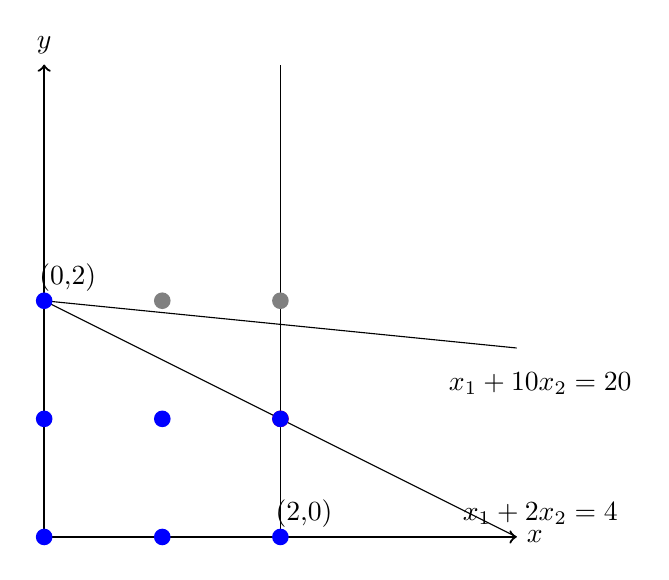
\begin{tikzpicture}[scale=1.5]
	% Draw axes
	\draw [<->,thick] (0,4) node (yaxis) [above] {$y$}
	|- (4,0) node (xaxis) [right] {$x$};
	% Draw two intersecting lines
	\draw (0,2) coordinate (a_1) -- (4,1.6) coordinate (a_2);
	\draw (4.2, 1.3) node {$x_1 + 10 x_2 = 20$};
	\draw (0,2) coordinate (a_1) -- (4,0) coordinate (a_2);
	\draw (4.2, 0.2) node {$x_1 + 2 x_2 = 4$};
	\draw (2,0) coordinate (b_1) -- (2,4) coordinate (b_2);
	% Calculate the intersection of the lines a_1 -- a_2 and b_1 -- b_2
	% and store the coordinate in c.
	\coordinate (c) at (intersection of a_1--a_2 and b_1--b_2);
	% Draw a dot to indicate intersection point
	\fill[red] (c) circle (2pt);
	\fill[blue] (0,0) circle (2pt);
	\fill[blue] (1,0) circle (2pt);
	\fill[blue] (2,0) circle (2pt);
	\draw (2.2, 0.2) node {(2,0)};
	\fill[blue] (0,1) circle (2pt);
	\fill[blue] (1,1) circle (2pt);
	\fill[blue] (2,1) circle (2pt);
	\fill[blue] (0,2) circle (2pt);
	\draw (0.2, 2.2) node {(0,2)};
	\fill[gray] (1,2) circle (2pt);
	\fill[gray] (2,2) circle (2pt);
      \end{tikzpicture}
      \caption{加了一個額外限制的放鬆線性規劃}
      \label{fig:cut_lp_relaxation}
    \end{center}
  \end{figure}
  加入之後,
  可解整數集並沒有變,
  但可解非整數集變了。
  一些非整數被$x_1 + 2 x_2 \leq 4$這條限制給切掉了。
  而放鬆線性規劃解出來的點(0,2)就正好是整數線性規劃的最佳解。 
  
  以上的例子闡釋了切平面方法的精神。
  我們的目的是不斷加入新的線性限制(也就是切平面)來讓
  \begin{enumerate}
    \item 可解整數集(Feasible Integer Set)維持不變
    \item 新的限制切掉一些非整數點,而得到比較小的可解集(Feasible Set)。我們希望比較小的可解集可以幫助我們找到比較好的整數解。
  \end{enumerate}
  至於如何找切平面?
  這通常要依靠問題的特殊結構來幫我們找到好的切平面,
  而非隨便切一刀。

  切平面方法其實不只可以用在線性規劃中,
  在一些不能微分的凸性最佳化(Convex Optimization)問題中也適用。
  而這正好就是我們的結構化支撐向量機要解的問題。 

  首先,
  我們注意到圖\ref{fig:active_constraint},
  \begin{figure}
    \subfloat{
    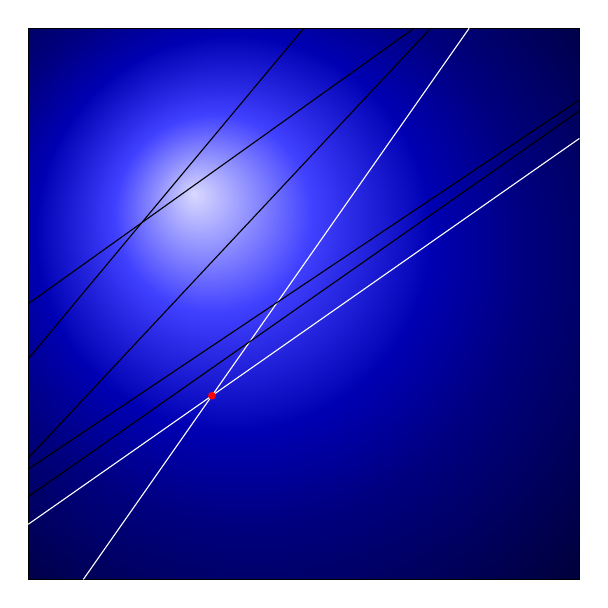
\begin{tikzpicture}[scale=0.7]
      \draw[ball color=blue,shading=ball] (0,0) rectangle (10, 10);
      \draw[white] (1,0) coordinate (a_1) -- (8,10) coordinate (a_2);
      \draw[white] (0,1) coordinate (b_1) -- (10,8) coordinate (b_2);
      \coordinate (c) at (intersection of a_1--a_2 and b_1--b_2);
      \fill[red] (c) circle (2pt);
      \draw (0,5) -- (7,10);
      \draw (0,4) -- (5,10);
      \draw (0,1.5) -- (10,8.5);
      \draw (0,2) -- (10,8.7);
      \draw (0,2.2) -- (7.3,10);
    \end{tikzpicture}
    }
    \subfloat{
    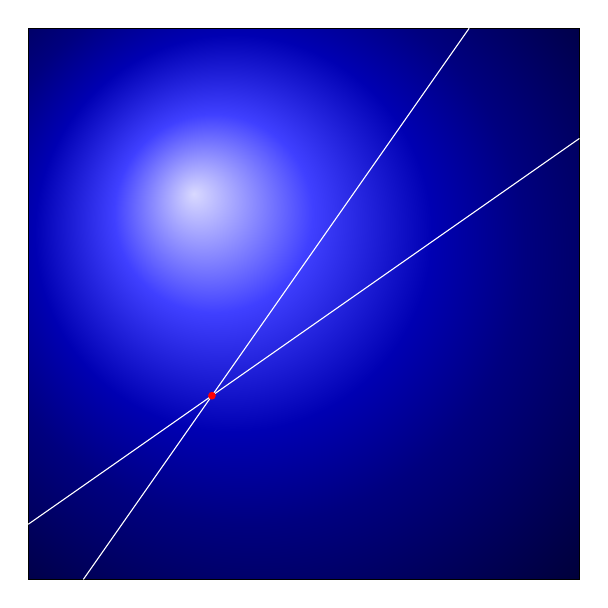
\begin{tikzpicture}[scale=0.7]
      \draw[ball color=blue,shading=ball] (0,0) rectangle (10, 10);
      \draw[ball color=blue,shading=ball] (0,0) rectangle (10, 10);
      \draw[white] (1,0) coordinate (a_1) -- (8,10) coordinate (a_2);
      \draw[white] (0,1) coordinate (b_1) -- (10,8) coordinate (b_2);
      \coordinate (c) at (intersection of a_1--a_2 and b_1--b_2);
      \fill[red] (c) circle (2pt);
    \end{tikzpicture}
    } 
    \caption{活性限制}
    \label{fig:active_constraint}
  \end{figure}
  圖中描述了一個凸性最小化的問題
  (顏色越淺表示值越小,顏色呈圓圈擴散是因為凸性函數,我們的目標就是距離白色點越近越好),
  雖然限制有一大堆(圖中的黑線加上白線,我們不能超過這些線),
  但真正有作用的限制是很少的(其實真正阻擋我們的是白線而非黑線),
  我們稱這些有作用的限制為活性限制(Active Constraint)。

  我們希望我們的結構化支撐向量機問題也能像圖\ref{fig:active_constraint}一樣有活性限制很少的性質,
  這樣我們解問題的時候就只要找出這些活性限制就好了。
  文獻中\cite{SVMstructJournal}證明,
  當我們定義的特徵函數$\Psi(x,y)$能使得$\Vert \Psi(x,y) - \Psi(x, \hat{y}) \Vert, \forall y, \hat{y} \in \mathcal{Y}$有多項式的上限,
  則活性限制的數量就具有多項式的上限。
  對於許多類型的問題,
  文獻中\cite{SVMstructJournal}已證明了有多項式上限,
  包括這本論文中所用的隱藏式馬可夫模型形式的結構化支撐向量機。

  只要活性限制有多項式上限,
  則我們便可以推出基於切平面方法的演算法\ref{alg:cutting_plane_svm_struct},
  並保證演算法\ref{alg:cutting_plane_svm_struct}可以在多項式時間內跑完。
  (因為活性限制只有多項式那麼多個)
  由演算法\ref{alg:cutting_plane_svm_struct}的第七行也可以知道,
  當演算法停止的時候,
  找出來的解會滿足所有活性限制到精準度$\epsilon$,
  也因此,
  所有限制(包括那些沒有被窮舉出來的限制)可以被保證不會被違反超過$\epsilon$。
  總結來說,
  我們便得到一個可以在多項式時間內保證所有限制不會被違反超過$\epsilon$的近似演算法。 
  
  以上大致簡介了演算法的正確性,
  詳細的證明請見\cite{SVMstructJournal}。
  接下來我們就大致說明一下演算法\ref{alg:cutting_plane_svm_struct}的過程。
  如果把整個演算法的過程圖示化的話,
  看起來就像圖\ref{fig:cutting_plane_proc}(圖中的圓圈是我們真正想要的限制,但因為它是非線性的,
  我們用線性限制條件逼近,好讓最後紅色點落在圓圈附近)。
  我們設定好成本函數之後(這決定了圖\ref{fig:cutting_plane_proc}中的顏色分佈),
  首先就是要找到違反最多的限制條件(Most-Violated Constraint),
  將它加到我們考慮的活性限制中(相當於圖\ref{fig:cutting_plane_proc}找出黑線可能的位置)。
  就相當於演算法第五行找到最大的$\hat{y}$,
  (因為在我們的問題中,
  每個$\hat{y}$就對應於一個限制,
  而找一個$\hat{y}$讓$H(y)$最大,
  就等於是找到違反最多的限制條件。
  且注意違反最多的限制一定是一個活性限制)

  接著,
  在第六行我們找出了現在的$\xi_i$(代表訓練錯誤的上限),
  如果違反最多的成本超過現在的$\xi_i$加上$\epsilon$的話(超出了訓練錯誤的上限表示我們一定還要加限制條件來切掉一塊區域),
  我們就把$\hat{y}$加進我們考慮的活性限制中(在圖\ref{fig:cutting_plane_proc}中將畫出一條新的黑線),
  並如切平面方法一般,
  重新計算我們的最佳化問題(在圖\ref{fig:cutting_plane_proc}中決定紅色的點新的位置),
  即重新解我們的支撐向量機對偶形式中的$\alpha$
  \begin{figure}
    \subfloat{
    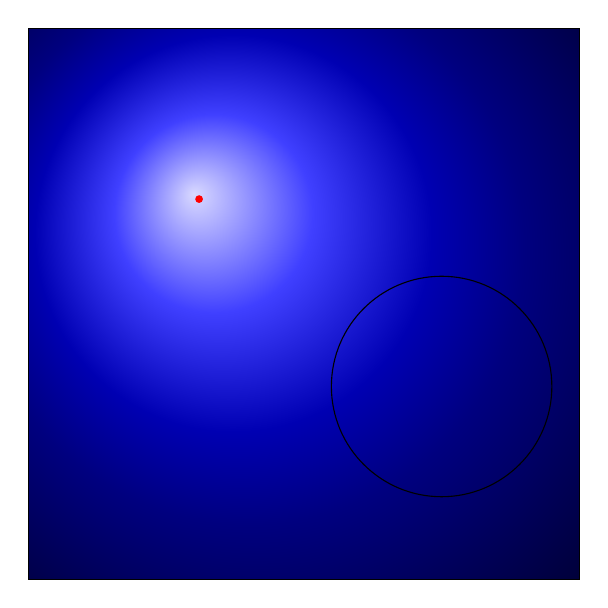
\begin{tikzpicture}[scale=0.7]
      \draw[ball color=blue,shading=ball] (0,0) rectangle (10, 10);
      \fill[red] (3.1,6.9) circle (2pt);
      \draw (7.5,3.5) circle (2);
    \end{tikzpicture}
    }
    \subfloat{
    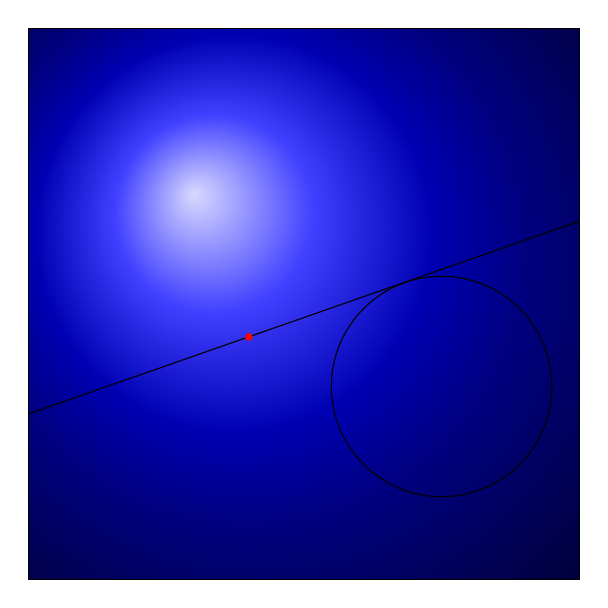
\begin{tikzpicture}[scale=0.7]
      \draw[ball color=blue,shading=ball] (0,0) rectangle (10, 10);
      \draw (7.5,3.5) circle (2);
      \draw (0,3) coordinate (a_1) -- (10,6.5) coordinate (a_2);
      \fill[red] (4,4.4) circle (2pt);
    \end{tikzpicture}
    } \\
    \subfloat{
    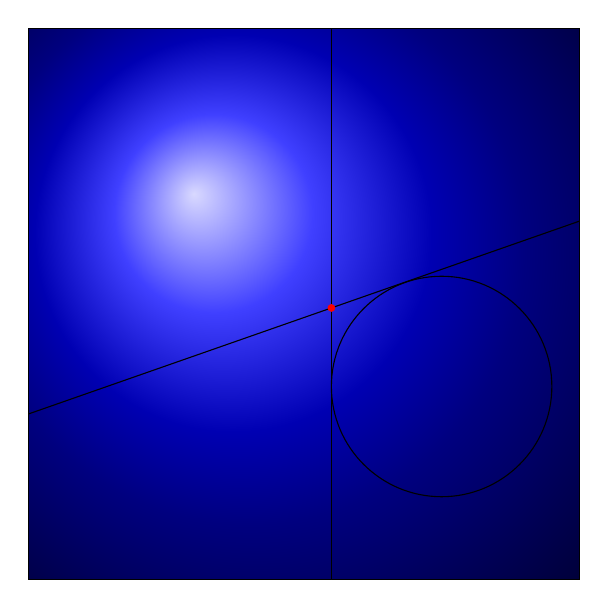
\begin{tikzpicture}[scale=0.7]
      \draw[ball color=blue,shading=ball] (0,0) rectangle (10, 10);
      \draw (0,3) coordinate (a_1) -- (10,6.5) coordinate (a_2);
      \draw (5.5,0) coordinate (b_1) -- (5.5,10) coordinate (b_2);
      \coordinate (c) at (intersection of a_1--a_2 and b_1--b_2);
      % Draw a dot to indicate intersection point
      \fill[red] (c) circle (2pt);
      \draw (7.5,3.5) circle (2);
    \end{tikzpicture}
    } 
    \subfloat{
    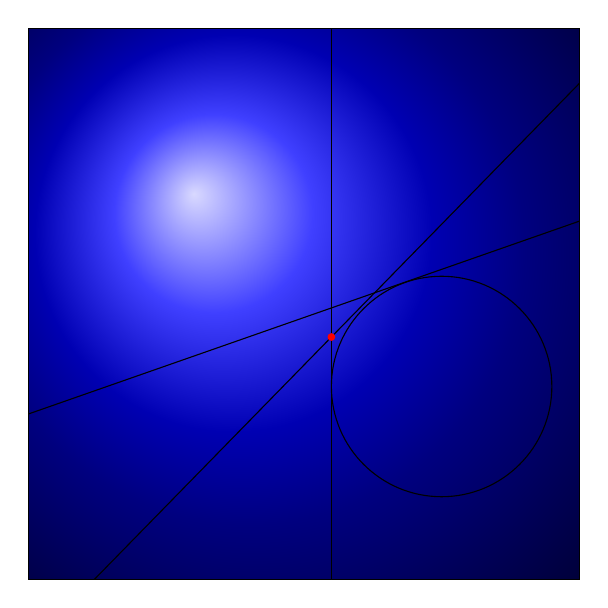
\begin{tikzpicture}[scale=0.7]
      \draw[ball color=blue,shading=ball] (0,0) rectangle (10, 10);
      \draw (0,3) coordinate (a_1) -- (10,6.5) coordinate (a_2);
      \draw (5.5,0) coordinate (b_1) -- (5.5,10) coordinate (b_2);
      \draw (1.2,0) coordinate (c_1) -- (10,9) coordinate (c_2);
      \coordinate (c) at (intersection of c_1--c_2 and b_1--b_2);
      % Draw a dot to indicate intersection point
      \fill[red] (c) circle (2pt);
      \draw (7.5,3.5) circle (2);
    \end{tikzpicture}
    } 
    \caption{切平面方法圖示}
    \label{fig:cutting_plane_proc}
  \end{figure}

  \begin{algorithm}
    \begin{algorithmic}[1]
      \STATE $S_i \leftarrow \emptyset \forall i = 1, \ldots, n$
      \REPEAT
	\FOR{$i = 1, 2 \dotsb, n$}
	  \STATE 建立成本函數$H(y) \equiv (1 - \langle \delta \Psi_i (y), w \rangle) \Delta(y_i, y)$
	  \STATE 計算$\hat{y} = \arg \max_{y \in \mathcal{Y}} H(y)$
	  \STATE 計算$\xi_i = \max \lbrace 0, \max_{y \in S_i} H(y) \rbrace$
	  \IF{$H(\hat{y}) > \xi_i + \epsilon$}
	    \STATE $S_i \leftarrow S_i \cup \lbrace \hat{y} \rbrace$
	    \STATE $\alpha_S \leftarrow$ 在$S$上面解對偶形式,其中$S = \cup_i S_i$
	  \ENDIF
	\ENDFOR
      \UNTIL{$S_i$不再變動}
    \end{algorithmic}
    \caption{SVM-struct切平面訓練演算法}
    \label{alg:cutting_plane_svm_struct}
  \end{algorithm}

\section{與鑑別式訓練法則之差異}
  由上述的介紹我們可以知道,
  結構化支撐向量機其實可以說是用極大化邊距原則(Large Margin Principle)來估測參數的條件隨機域(Conditional Random Field)模型,
  屬於鑑別式模型(Discriminative Model)。
  將鑑別式模型應用在語音辨識上,
  我們很自然地會聯想到同樣有「鑑別」兩個字的鑑別式訓練法則(Discriminative Training)。
  它們似乎都是想要將我們要的詞串跟其他競爭詞串拉開,
  究竟它們之間的關係是什麼?
  是可以比較還是不能比較?

  根據文獻\cite{modelVStraining}的推導,
  鑑別式訓練法則其實就是一種鑑別式模型。
  但由於現今的鑑別式訓練模型都是從重新定義貝氏風險(Bayes Risk)出發推導出來的,
  所以數學形式上屬於貝氏學派(Bayesian School)的鑑別式模型,
  而非統計學派(Statistical School)的鑑別式模型,
  也就是說跟邏輯迴歸(Logistic Regression)、
  線性判別分析(Linear Discriminant Analysis)、
  支撐向量機(Support Vector Machine)等模型的數學形式不太一樣。
  至於鑑別式訓法則能不能跟鑑別式模型比較呢?
  答案是可以,
  就像我們會將支撐向量機與邏輯迴歸比較一樣,
  既然鑑別式訓練法則被推導出其實是鑑別式模型,
  當我們想要驗證不同鑑別式模型針對某個問題的適用性時,
  就可以將它們一一拿來跑實驗。
  只是,
  由於不同問題結構不一樣,
  可能在不同問題上不同鑑別式模型有不同的表現。
  舉語音辨識的例子來講,
  採用貝氏學派方法的鑑別式訓練法則,
  可以有效拆解語音辨識這個複雜的問題。
  所以相較於其他比較年輕的鑑別式模型像是條件隨機域、結構化支撐向量機等等,
  已經有辦法應用在大字彙辨識的問題上。
  而條件隨機域、結構化支撐向量機雖然理論上是可行,
  但目前還沒有人找出可以有效應用在大字彙辨識上。

  由於這一章是在介紹結構化支撐向量機,
  所以特別值得一提的是有一種鑑別式訓練法則跟結構化支撐向量機的形式有點像,
  它叫做極大邊距隱藏式馬可夫模型(Large Margin HMM) \cite{LargeMarginHMM}。
  它用的原則也是「將第一名與第二名之間的邊距盡量拉開」。
  不過它原則套用的方式跟結構化支撐向量機不一樣,
  極大邊距隱藏式馬可夫模型是套用鑑別式訓練法則的架構,
  將每個字或音素所對應的隱藏式馬可夫模型間的邊距拉開。
  (跟最小分類錯誤訓練法不同,
  最小分類錯誤訓練法是將不同隱藏式馬可夫模型間的邊距盡量都變成正的,
  而極大邊距隱藏式馬可夫模型是不只要變成正的,
  還要極大化邊距)
  但結構化支撐向量機要拉開的邊距則是正確音素串跟錯誤音素串之間的距離。
  同樣作為鑑別式模型,
  很自然會想要將極大邊距馬可夫模型跟結構化支撐向量機做比較。
  不過就現階段來講,
  就像拿結構化支撐向量機跟鑑別式訓練法則比較一樣,
  目前結構化支撐向量機還是個年輕的模型,
  在結構上也還沒有人嘗試出能有效拆解語音辨識問題的結構,
  所以在效能上是不及鑑別式訓練法則的。
  自然跟極大化邊距隱藏式馬可夫模型比較也一定會輸。

  結構化支撐向量機跟極大化隱藏式馬可夫模型是兩個原則相同但不同路線的兩個模型,
  都十分複雜也同樣都有進步空間,
  像兩個模型同樣都用到逼近(Approximation)演算法,
  而且極大化隱藏式馬可夫模型逼近時要放鬆的假設也比結構化支撐向量機要多上不少。
  且極大化隱藏式馬可夫模型目前也只做到TI Digit這套測試語料
  (不同數字的辨識),
  還沒有人成功將它套用到大字彙辨識上。

\section{本章總結}
  結構化支撐向量機是最近機器學習領域所提出的一種新的模型框架,
  只要對模型夠了解,
  更改其中的$\Psi(x,y)$的結構就可以使用在不同的結構性輸出問題上。
  因此衍生出不少的變形,
  有人拿來做解析(Parsing),有人拿來做資訊檢索(Information Retrieval)。
  而本章對於他的框架及訓練演算法做了基本的探討。
